\chapter{Experiment Setup}
\section{ASK Configuration}

\subsection{Introduction: ASK Module Pipeline}

ASK's flexibility and extensibility come from its modular architecture. When running an experiment, ASK follows the pipeline below,


\begin{center}
  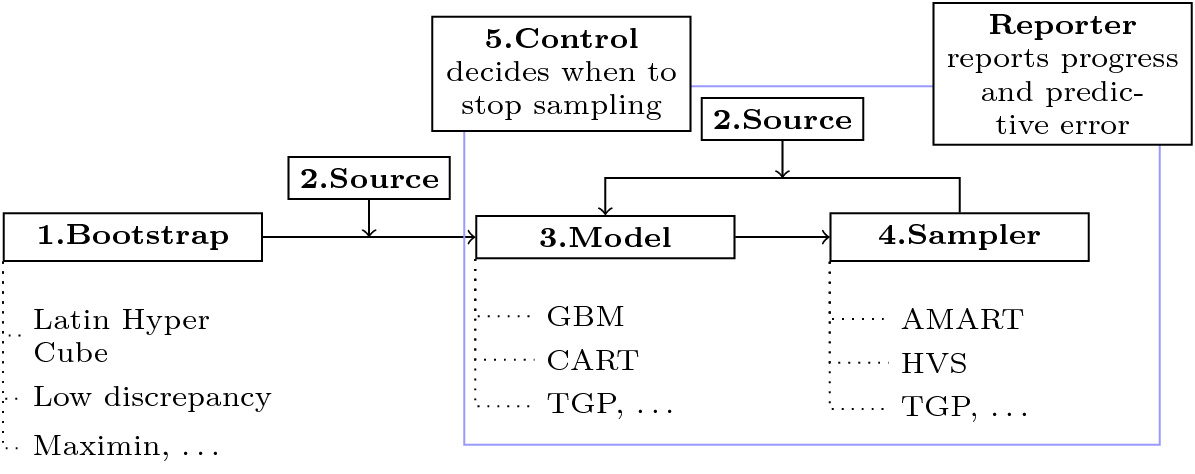
\includegraphics[width=\textwidth]{figures/ASK-modules-pipeline.png}
\end{center}


First, the \textbf{Bootstrap} module selects a set of initial points to measure. The initial selection is passed to the \textbf{Source} module which runs an experiment for each point and returns the measured response. A \textbf{Model} module fits the first set of measures to a surrogate model, producing a first prediction of the response on the full design space. Since the prediction is still very rough, the \textbf{Sampler} modules chooses additional points to measure that will improve the model accuracy. The sampler selected points are measured with the \textbf{Source} module and fitted again in the model.
The \textbf{Control} module is in charge of stopping the process after a fixed number of iteration or when a quality threshold is reached. Finally, the \textbf{Reporter} module produces informative statistics for the user during the experiment.

ASK offers different implementations for each module. It allows building customized experimental pipelines. If one feature is missing, users can write their own module implementing it.

\subsection{ASK invocation}

The coordination between the modules is entirely handled by ASK. 
Before running an experiment, the user must prepare a configuration file describing the experiment's parameters and the selected modules.
Once the configuration file is ready, the user should type,

\begin{minted}{bash}
$ ask <configuration_file>
\end{minted}

Any fatal error stops the execution and is immediately reported to the user. Warnings are logged to a log file. By default the log file name is \texttt{default.log}. All the samples measured, models built and reports produced are saved inside an output directory, which is by default called \texttt{output/}. The configuration file allows changing both the log file name and the output directory names.

The following command line flags alter the default behavior:

\begin{itemize}
	\item \texttt{-h} or \texttt{--help}, returns a short message describing the available flags and their usage.
	\item \texttt{--force\_overwrite}, to prevent accidental loss of experiment data, ASK refuses to run if the output directory already exist in the current path. If this option is used ASK will overwrite the previous output directory with the new experiments.
	\item \texttt{--skip\_reporter}, this flag runs an ASK experiment by skipping calls to the Reporter module. This is useful for long runs on which the user will not supervise the execution and wants to avoid the overhead of generating reports.
	\item \texttt{--skip\_model}, this flag runs an ASK experiment by skipping calls to the Model module. Beware; if the Reporter or Sampler module you use require a surrogate model, using this flag will raise an error at execution.
	\item \texttt{--replay\_only}, this flag requires that a previously created output directory exists. It replays a previous ASK experiment bypassing calls to the source, sampler, and bootstrap modules. This enables reusing old measures with a new reporter or model module. A common scenario for this flag is doing experiments on a remote machine, where calling the reporter module is unnecessary, retrieving the data on the experimenter's local computer, and replaying the experiments with the reporter module enabled to analyze the results.
\end{itemize}

\begin{minted}{bash}
$ ./ask -h
usage: ask [-h] [--force_overwrite] [--replay_only] [--skip_model]
           [--skip_reporter]
           configuration

Helps choosing sampling points during experiments.

positional arguments:
  configuration      the experiment configuration file

optional arguments:
  -h, --help         show this help message and exit
  --force_overwrite  If a previous output directory is found its contents will
                     be overwritten
  --replay_only      (Must be run over a full previous ask run). Skip
                     bootstrap and sampler modules, but runs previous labels
                     through the model and reporter. This option is useful if
                     one wants to run sampling and analyze results separately.
  --skip_model       Skip model module. (WARNING: if the chosen control module
                     relies on the output of the model module, this option
                     fails.)
  --skip_reporter    Skip reporter module. (WARNING: if the chosen control
                     module relies on the output of the reporter module, this
                     option fails.)
\end{minted}

\subsection{ASK Configuration File}

This section describes the ASK configuration file format. The ASK configuration file follows the \href{http://www.json.org/}{JavaScript Object Notation (JSON)} format. The simple example of \hrefinternal{http:///wiki/Application_Characterization:_ASK:_Chapter_2:_Installation_and_First_Use}{Chapter 2} is presented below.

\begin{minted}{js}
{
  "factors": [
    {"name": "x",
     "type": "integer",
     "range": {"min": -200, "max": 600}
    },
    {"name": "y",
     "type": "integer",
     "range": {"min": -200, "max": 600}
    }
  ],
  "modules": {
    "bootstrap": {
      "executable": "bootstrap/random",
      "params": {        
        "n": 500
      }
    },
    "source": {
      "executable": "source/file",
      "params": {
        "data_file": "gauss2D.data"
      }
    },
    "model": {
      "executable": "model/gbm_build",
      "predictor": "model/gbm_predict",
      "params": {"ntrees":100, "interactiondepth": 5, "shrinkage":0.1}
    },
    "sampler": {
      "executable": "sampler/hierarchical",
      "params": {
        "cp":0.01,
        "n":50,
        "ponderate_by_size":false
      }
    },
    "control": {
      "executable": "control/points",
      "params": {
        "n": 500
      }
    },
    "reporter": {
      "executable": "reporter/generic/report",
      "params": {
        "test_set": "gauss2D.data",
        "max_error_scale": 1,
        "timeseries": "simple_timeseries.out",
        "script": "reporter/generic/2D.R"
      }
    }
  },
  "log": {
    "logfile": "default.log",
    "level": "DEBUG"
  },
  "output_directory": "output/"
}
\end{minted}

There are four outer level sections:
\begin{itemize}
	\item \texttt{output\_directory} specifies the name of the output directory.
	\item \texttt{log} specifies the name of the log file and the log level. There are five log levels: DEBUG, INFO, WARNING, ERROR, and CRITICAL. The higher the log level the less messages are logged.
	\item \texttt{factors} section configures the experiment's factors.
	\item \texttt{modules} section configures the modules.
\end{itemize}

Factors and most modules sections are mandatory. Nevertheless, some sections are optional: output\_directory, log, modules.model, and modules.reporter. Sane default values replace optional missing sections, the default values can be changed by editing the file \texttt{ask/default.conf}. 

\subsubsection{Factors Section}

The factors section describes each of the factors, sometimes called independent variables, of your experiment.
Each factor can take different values. The response, sometimes called dependent variable, will be measured and 
predicted for different combinations of the factors values.

Below is a factors section demonstrating all the different types of factors available in ASK.

\begin{minted}{js}
"factors": [
  {"name": "number_of_threads",
  "type": "integer",
  "range": {"min": 1, "max": 32}
  },
  {"name": "seed",
  "type": "float",
  "range": {"min": -10.3, "max": 3.1415}
  },
  {"name": "cache_level",
  "type": "categorical",
  "values": ["L1", "L2", "L3"]
  },
],
\end{minted}

The factors section is an array of factors. Each factor is an object with three attributes:
\begin{itemize}
	\item \texttt{name}, contains a unique string identifying the factor.
	\item \texttt{type}, describes the type of factor. There are three valid types:
	\begin{itemize}
		\item \texttt{integer}, represent an integer factor bounded by a minimum and maximum value.
		\item \texttt{float}, represents a real factor bounded by a minimum and maximum value.
		\item \texttt{categorical}, represents a discrete factor that can take a finite number of categorical values. No order is assumed among the values.
	\end{itemize}
	\item The third attribute determines the admissible values for the factor. The name of the third attribute depends on the type of factor. For \texttt{integer} or \texttt{float} types the third attribute is \texttt{range}; for \texttt{categorical} type, the third attribute is \texttt{values}.
	\begin{itemize}
		\item \texttt{range}, is an object with two attributes \texttt{min} and \texttt{max} giving the inclusive lower and upper bounds of the factor.
		\item \texttt{values}, is an array of strings. Each string corresponds to a possible value of the categorical factor.
	\end{itemize}
\end{itemize}

\subsubsection{Modules Section}

The module section selects for each module one specific implementation and if needed configures the module parameters.

\begin{minted}{js}
"modules": {
  "bootstrap": {
    "executable": "bootstrap/random",
    "params": {
      "n": 500
    }
  },
  "control": {
    "executable": "control/points",
    "params": {
      "n": 500
    }
  },
  "reporter": {
    "executable": "reporter/generic/report",
    "params": {
      "test_set": "gauss2D.data",
      "max_error_scale": 1,
      "timeseries": "simple_timeseries.out",
      "script": "reporter/generic/2D.R"
    }
  },
  "source": {
    "executable": "source/file",
    "params": {
      "data_file": "gauss2D.data"
    }
  },
  "sampler": {
    "executable": "sampler/hierarchical",
    "params": {
      "cp":0.01,
      "n":50,
      "ponderate_by_size":false
    }
  },
  "model": {
    "executable": "model/gbm_build",
    "predictor": "model/gbm_predict",
    "params": {"ntrees":100, "interactiondepth": 5, "shrinkage":0.1}
  }
},
\end{minted}

The order of the modules instantiations is not important.
Each module subsubsection contains two parameters:
\begin{itemize}
	\item \texttt{executable}, which contains the path of the module's chosen instance. Each instance is an executable file. The path can be absolute or relative to the current directory or to ASK's root directory; path resolution proceeds in this exact order.
	\item \texttt{params}, contains a list of module specific parameters. The format of \texttt{params} is module dependent, \hrefinternal{http:///wiki/Application_Characterization:_ASK:_Chapter_4:_Standard_Modules}{Chapter 4} describes the parameters expected by each module.
\end{itemize}

Model modules are an exception. Indeed, a model module responsibilities are two-fold:
\begin{itemize}
	\item building models from sampled data
	\item predicting the response on new data
\end{itemize}

The model subsubsection expects the executable for building a model in the \texttt{executable} field. It contains an additional parameter, 
\texttt{predictor} that gives the path of the module's predictor path.

\subsection{Data Exchange Format}

This section describes the format used by ASK modules to exchange points and their response.
The format is in space separated values format.
Let \textbf{n} be the number of factors declared in the \hrefinternal{http:///wiki/Application_Characterization:_ASK:_Chapter_3:_Experiment_Setup\#ASK_Configuration_File}{Factors section} of the configuration file.

Each line of the file represents a point in the space. The first \textbf{n} columns represent the factor values in the order of the \hrefinternal{http:///wiki/Application_Characterization:_ASK:_Chapter_3:_Experiment_Setup\#ASK_Configuration_File}{Factors section}. If a \textbf{n+1} column is added, it represents the response measured for this factor combination.

The file below contains four points, the first five columns are the factors coordinates, and the sixth column contains the response:

\begin{minted}{bash}
1 64 64 0 4 109.728
12 314 1064 4 0 9.14235
1 314 1064 4 1 115.078
4 564 64 0 0 9.01366
\end{minted}

\section{Setting Up an Experiment}

This section explains systematically how to setup an ASK experiment using the 2D synthetic design space that was used in \hrefinternal{http:///wiki/Application\_Characterization:\_ASK:\_Chapter\_2:\_Installation\_and\_First\_Use\#First\_Use}{Chapter 2}:


$$
f(x_1,x_2) = \frac{x_1}{100}.e^{-(\frac{x_1}{100})^2-(\frac{x_2}{100})^2} \textrm{ on } [-200:600] \times [-200:600]
$$

The design space is inspired by an example from the article, \emph{tgp: An R package for Bayesian nonstationary, semiparametric nonlinear regression and design by treed gaussian process models}, R.B. Gramacy, Journal of Statistical Software 2007. 
The design space has two factors x1 and x2 and the response plotted below.

\begin{center}
  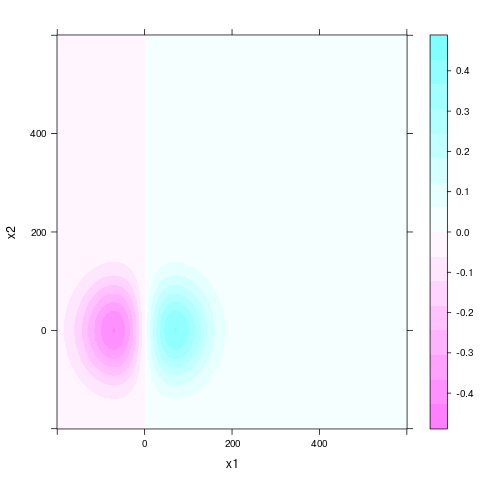
\includegraphics[width=\textwidth]{figures/ASK-gauss2D-ideal.png}
\end{center}



The configuration and set-up described below is available in the directory \texttt{ask/examples/gauss2D}.

\subsection{Writing a Source Module}

The first step is defining a source module to measure the response on any point of the space.
In the example, the module simply computes the response of the function f over the input points.
Below is a simple R implementation for the source module:

\begin{minted}{r}
#!/usr/bin/env Rscript
# A simple source module
# Parse the module arguments
args <- commandArgs(trailingOnly = T)
if (length(args) != 3) {
    stop("Usage: source <configuration.conf> <requested_file> <output_file>")
}

# Read the requested points
requested = read.table(args[2])

# Define the function to study
# (A real experiment would here call some measurement process)
myf <- function (x1,x2) {
  x1 = x1/100
  x2 = x2/100
  return (x1 * exp(-x1*x1 - x2*x2))
}

# Compute f over all the requested points
requested$response = myf(requested$V1, requested$V2)

# Write results
write.table(requested, args[3], sep=" ", quote=F, col.names=F, row.names=F)
\end{minted}

All \hrefinternal{http:///wiki/Application_Characterization:_ASK:_Chapter_5:_Writing_Modules\#Source_Modules}{source modules} take three arguments:
\begin{enumerate}
	\item The path of the experiment \hrefinternal{http:///wiki/\#ASK_Configuration_File}{configuration file}.
	\item The path of the requested points file. This file contains the list of space points to be measured, in \hrefinternal{http:///wiki/\#Data_Exchange_Format}{ASK's data exchange format}.
	\item The path of the output file.
\end{enumerate}

The above script conforms to this interface: first, it parses the three arguments. Then, it reads the list of points to measure. Conveniently, the data exchange format used by ASK can be read from R with the \texttt{read.table()} function. For each combination of factors \texttt{(x1,x2)}, the response is computed. Finally, the script writes each combination and its response to the output file.
The above source module is straightforward and does not need additional configuration; therefore, it ignores the configuration file parameter.

Checking that the above implementation works is simple. Prepare a requested file with a few points, for instance:

\begin{minted}{bash}
<file: some.data>
10 10 
50 -15.3 
200 -30 
\end{minted}

Prepare an empty configuration file, for now.
Then call the source module on this file:

\begin{minted}{bash}
$./source.R empty.conf some.data out.data
$cat out.data
10 10 0.0980198673306755
50 -15.3 0.3803907821641490
200 -30 0.0334784671171613
\end{minted}

As expected, the source module computes the response for each factor.
The source module is the interface between ASK and the user's experimental setup. The next section explains how to configure the rest of the experimental pipeline.

\subsection{Configuring the Factors}

To configure the experiment, write a \hrefinternal{http:///wiki/Application_Characterization:_ASK:_Chapter_3:_Experiment_Setup\#ASK_Configuration_File}{configuration file}.
Start with the \hrefinternal{http:///wiki/Application_Characterization:_ASK:_Chapter_3:_Experiment_Setup\#Factors_section}{Factors section} that describes the type and domain of the factors. The function f is defined on two float factors ranging from -200 to 600:

\begin{minted}{js}
"factors": [
  {"name": "x1",
   "type": "float",
   "range": {"min": -200, "max": 600}
  },
  {"name": "x2",
   "type": "float",
   "range": {"min": -200, "max": 600}
  }
],
\end{minted}

\subsection{Choosing and Configuring the Sampling Pipeline}

The next step is choosing and configuring the modules for the experiment.
One module must be chosen for each step of the \hrefinternal{http:///wiki/Application_Characterization:_ASK:_Chapter_3:_Experiment_Setup\#Introduction:_ASK_module_pipeline}{experimental pipeline}.

\subsubsection{Source Module}

First add the \hrefinternal{http:///wiki/\#Writing_a_Source_Module}{source module} that measures f. Remember, it is a simple R executable, called \texttt{source.R}.
\begin{minted}{js}
"modules": {
  "source": {
    "executable": "./source.R",
    "params": {}    
  }
}
\end{minted}

The script does not expect any configuration parameters so \texttt{"params"} is left empty.
Remember to set the executable bit of source.R before running the experiment.

\subsubsection{Bootstrap Module}

The bootstrap module selects the first batch of sampled points. ASK offers different standard bootstrap modules available in the \texttt{ask/bootstrap} directory and described in \hrefinternal{http:///wiki/Application_Characterization:_ASK:_Chapter_4:_Standard_Modules}{Chapter
4: Standard Modules}.

The example uses the \texttt{bootstrap/random} module that selects random factor combinations.

\begin{minted}{js}
"bootstrap":  {
  "executable": "bootstrap/random",
  "params": {"n": 50}
}
\end{minted}

The parameter \texttt{"n"} specifies that exactly 50 combinations should be sampled during bootstrap.

\subsubsection{Model Module}

The model module predicts the response in locations not yet sampled.
The example uses the \href{http://cran.r-project.org/web/packages/gbm/}{Generalized Boosted Model} with its default parameters.

\begin{minted}{js}
"model":  {
  "executable": "modules/gbm_build",
  "predictor": "model/gbm_predict",
  "params": {}
}
\end{minted}

When no parameters are specified, default values are provided.
GBM works by combining multiple tree predictors, the default number of trees is 3000.
To change this value to 1000, one would simply use the line:

\begin{minted}{js}
"params": {"ntrees":1000}
\end{minted}

\hrefinternal{http:///wiki/Application_Characterization:_ASK:_Chapter_4:_Standard_Modules}{Chapter 4: Standard Modules} describes the full set of available configuration.

\subsubsection{Sampler Module}

The sampler module samples additional points for every iteration of the experimental pipeline.
The examples uses the Hierarchical Variance Sampler included in ASK and samples 50 new points per iteration.

\begin{minted}{js}
"sampler": {
  "executable": "sampler/hierarchical",
  "params": {"n": 50}
}
\end{minted}

\subsubsection{Control Module}

The control module chooses when to end the experiment. The example uses the \texttt{points} control, which stops after a given number of points in sampled.

\begin{minted}{js}
"control": {
  "executable": "control/points",
  "params": {"n": 500}
}
\end{minted}

Here the experiment will stop after sampling 500 points, which amounts to one bootstrap sampling and nine Hierarchical Variance samplings.

\subsubsection{Report Module}

The report module produces detailed statistics about the sampling.
In this case, the generic reporter is used:

\begin{minted}{js}
"reporter": {
  "executable": "reporter/generic/report",
  "params": {
    "script": "reporter/generic/2D.R",
    "test_set": "test.data",
    "timeseries" : "timeseries.out"
  }
}
\end{minted}

The \texttt{script} parameter requires a script to plot the response prediction. ASK includes default scripts to handle 1D and 2D dimensions.
For higher dimensions, users must provide their own script.

The \texttt{test\_set} parameter is the path of a file containing a set of measures to use as a test set in \hrefinternal{http:///wiki/\#Data_Exchange_Format}{ASK's data exchange format}.

Finally, \texttt{timeseries} parameter is the path of an output file. The generic reporter module produces in this file the time series of the model accuracy. Plotting this time series is interesting to evaluate if the model converges.

\subsection{Running the Experiment}

To run the experiment type:

\begin{minted}{bash}
$ ask experiment.conf
Logging to default.log
Experiments finished normally
\end{minted}

A trace of all the modules messages is logged in the log file, \texttt{default.log}.

\subsection{Analyzing the Experiment}

Once the experiment is finished you can visualize the evolution of the model by displaying the files \texttt{output/plot0000?.png}.
The \texttt{?} should be substituted by an iteration number. Bootstrap iteration is number 0.
The first level plot shows the error across x1 and x2. The second level plot shows the model prediction across x1 and x2.
The circles mark the sampled positions. The red circles mark the positions sampled in the current iteration, for instance red circles
in \texttt{output/plot00009.png} show the points sampled in the last iteration.

\begin{center}
  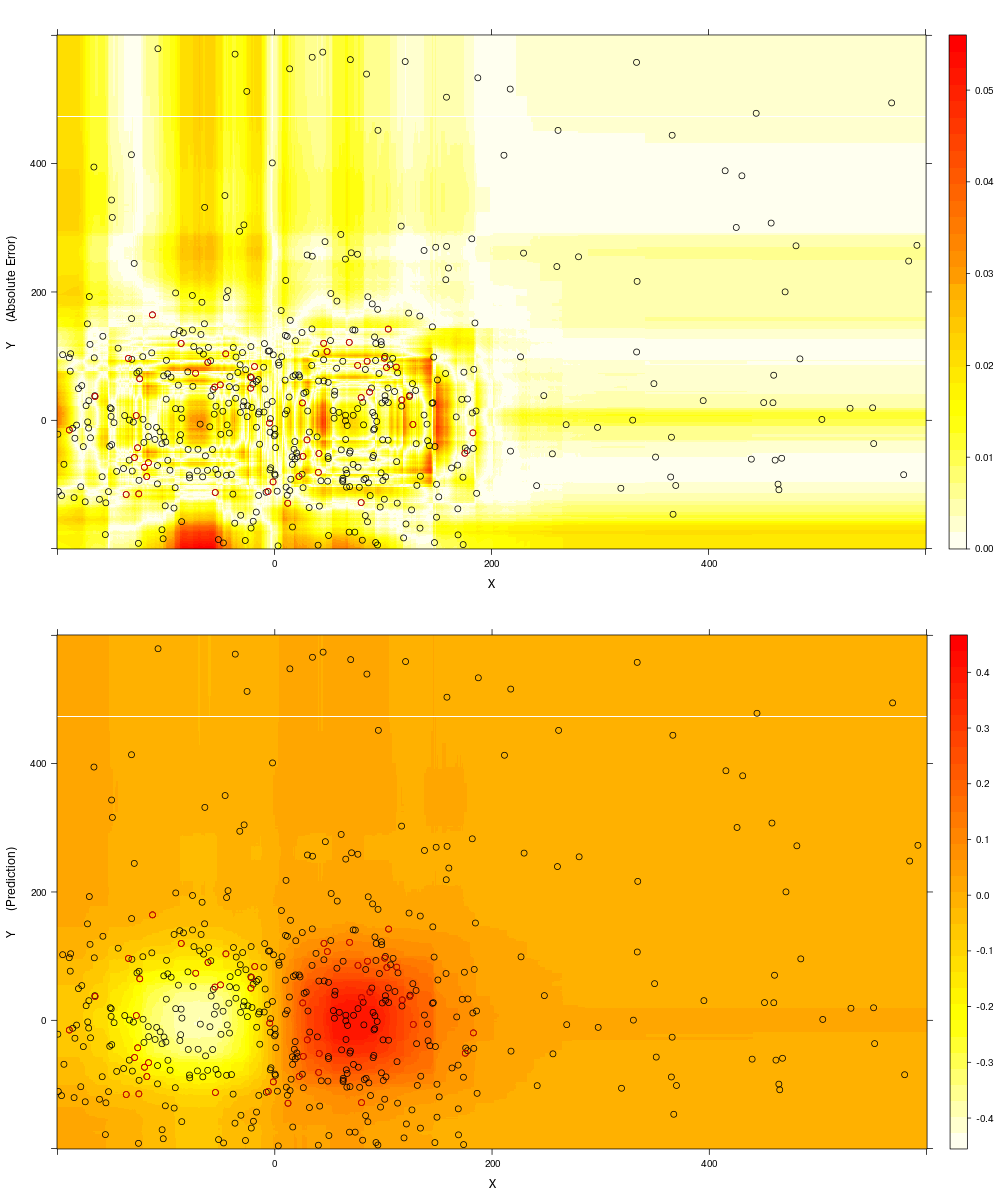
\includegraphics[width=\textwidth]{figures/ASK-gauss-levelplot.png}
\end{center}



The time series file contains the following values:
\begin{minted}{bash}
samples mean-error max-error rmse mean-relative max-relative
50 0.0377823384121497 0.447323111968324 0.0781095183475204 Inf Inf
100 0.0294159657374007 0.408494500075275 0.0630672408986823 Inf Inf
150 0.0275319895231202 0.281661273924844 0.0469645301362225 Inf Inf
200 0.0232192159241306 0.239290251332769 0.0376329805089173 Inf Inf
250 0.0174217850030764 0.142481821968832 0.0272243696109088 Inf Inf
300 0.0120016612421342 0.0846704149994422 0.0179698102164841 Inf Inf
350 0.00993725543490917 0.083600182129529 0.014940974890969 Inf Inf
400 0.00860058449418072 0.061942979615955 0.0124781071557198 Inf Inf
450 0.00835631286507885 0.0675461324475211 0.0126914309137798 Inf Inf
500 0.00787049320164634 0.0714181540783402 0.0119012098836963 Inf Inf
\end{minted}

The first column gives the number of samples; the following columns give the mean error of the model, the maximum error, the Root Mean Square Error (RMSE), the mean relative error, and the max relative error. The errors quantify the difference between the model prediction and the test set provided.
In this particular design space, since f can become 0, for example f(0,-200) = 0, the relative error is by definition undefined.

ASK includes a utility to plot the error time series:
\begin{minted}{bash}
$ <ask directory path>/utils/compare-time-series plot.png timeseries.out
\end{minted}

\begin{center}
  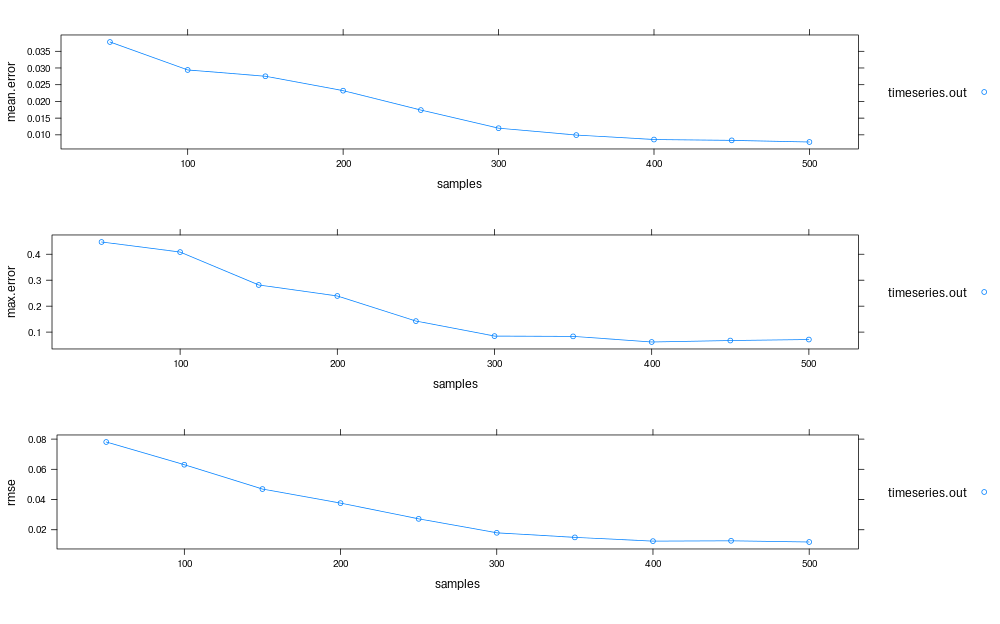
\includegraphics[width=\textwidth]{figures/ASK-gauss-timeseries.png}
\end{center}

The script is also useful to compare the accuracy of different configurations. Suppose different values are tried for the number of trees of the GBM model. For each configuration, experiments are rerun producing a new time series output \texttt{timeseries1.out, timeseries2.out, ...} 

Typing, 
\begin{minted}{bash}
$ <ask directory path>/utils/compare-time-series plot.png \
      timeseries1.out timeseries2.out [...]
\end{minted}

overlaps the error plots of each configuration.

Most sampling strategies included in ASK use random seeds. To evaluate precisely the behavior of one sampling strategy, it is recommended to take the median of multiple runs. The script \texttt{utils/merge-time-series} merges a set of individual time series by taking the median among all runs:
\begin{minted}{bash}
$ <ask directory path>/utils/merge-time-series aggregated.out \
      timeseries1.out timeseries2.out [...]
\end{minted}

\subsection{Reusing the Model}

Once ASK generates an accurate model, it can be used to predict any point in the exploration space. The model generated in the last iteration is \texttt{output/model00009.data}.

The model is able to predict the response for any new value. First, prepare a file with the desired combinations, for example:
\begin{minted}{bash}
<file: some.data>
10 10
50 -15.3
200 -30
\end{minted}

Then type:
\begin{minted}{bash}
$ export ASKHOME=<ask directory>; export PYTHONPATH=$ASKHOME:$PYTHONPATH
$ $ASKHOME/model/gbm_predict experiment.conf output/model00009.data \
    some.data prediction.data
$ cat prediction.data
10 10 0.098377986754355
50 -15.3 0.378151609613139
200 -30 0.0486711827411655
\end{minted}

Usually, the \texttt{ask} driver exports the two environment variables \texttt{ASKHOME} and \texttt{PYTHONPATH} automatically. In this example, the \texttt{gbm\_predict} module is called directly, therefore the two environment variables must be exported manually.

The predicted values can be compared with the true f values:

\begin{minted}{bash}
$  ./source.R experiment.conf some.data true.data
$ cat true.data
10 10 0.0980198673306755
50 -15.3 0.3803907821641490
200 -30 0.0334784671171613
\end{minted}

The prediction was very close for the first two points and less good for the last. 

